\documentclass[12pt,a4paper]{article}

% ─── Page Layout ───────────────────────────────────────────────────────────────
\usepackage[a4paper, margin=0.8in, headheight=14pt]{geometry}

% ─── Fonts (XeLaTeX) ───────────────────────────────────────────────────────────
\usepackage{fontspec}
\usepackage{unicode-math}
\setmainfont{TeX Gyre Pagella}
\setmonofont[Scale=0.88]{TeX Gyre Cursor}
\setmathfont{Latin Modern Math}

% ─── Packages ──────────────────────────────────────────────────────────────────
\usepackage{xcolor}
\usepackage{colortbl}
\usepackage{titlesec}
\usepackage{enumitem}
\usepackage{tabularx}
\usepackage{booktabs}
\usepackage{array}
\usepackage{amsmath}
\usepackage{tikz}
\usetikzlibrary{shapes.geometric, arrows.meta, positioning, calc, fit, decorations.pathreplacing}
\usepackage{tcolorbox}
\tcbuselibrary{skins, breakable}
\usepackage{hyperref}
\usepackage{fancyhdr}
\usepackage{graphicx}
\usepackage{microtype}
\hyphenpenalty=10000
\exhyphenpenalty=10000
\sloppy
\usepackage{caption}
\usepackage{setspace}
\usepackage{multirow}
\usepackage{tocloft}

% ─── Q&A helper ────────────────────────────────────────────────────────────────
\newcommand{\Q}[1]{\textbf{#1}\par\noindent\ignorespaces}

% ─── Colour Palette ────────────────────────────────────────────────────────────
\definecolor{myred}{RGB}{196,30,58}
\definecolor{mydark}{RGB}{30,30,50}
\definecolor{mygreen}{RGB}{14,120,80}
\definecolor{myteal}{RGB}{0,130,140}
\definecolor{myamber}{RGB}{180,100,0}
\definecolor{mypurple}{RGB}{100,30,160}
\definecolor{mygray}{RGB}{246,247,249}
\definecolor{mgframe}{RGB}{180,185,200}
\definecolor{watermark}{RGB}{145,150,170}
\definecolor{hdrred}{RGB}{250,232,235}
\definecolor{hdrgreen}{RGB}{220,244,233}
\definecolor{hdrteal}{RGB}{220,242,244}
\definecolor{hdramber}{RGB}{253,242,215}
\definecolor{hdrpurple}{RGB}{238,228,255}

% ─── Section Formatting ────────────────────────────────────────────────────────
\titleformat{\section}
  {\large\bfseries\color{myred}}{\thesection.}{0.5em}{}
  [\vspace{1pt}{\color{myred}\rule{\linewidth}{0.8pt}}]
\titleformat{\subsection}
  {\normalsize\bfseries\color{myteal}}{\thesubsection}{0.5em}{}
\titlespacing*{\section}{0pt}{18pt}{7pt}
\titlespacing*{\subsection}{0pt}{11pt}{4pt}

% ─── Paragraph ─────────────────────────────────────────────────────────────────
\setlength{\parindent}{0pt}
\setlength{\parskip}{4pt}

% ─── TOC Styling ───────────────────────────────────────────────────────────────
\renewcommand{\cfttoctitlefont}{\large\bfseries\color{myred}}
\renewcommand{\cftaftertoctitle}{\par\noindent{\color{myred}\rule{\linewidth}{0.8pt}}}
\setlength{\cftbeforetoctitleskip}{0pt}
\setlength{\cftaftertoctitleskip}{6pt}
\renewcommand{\cftsecfont}{\normalsize\bfseries\color{mydark}}
\renewcommand{\cftsecpagefont}{\normalsize\bfseries\color{mydark}}
\renewcommand{\cftsecleader}{\cftdotfill{\cftdotsep}}
\setlength{\cftbeforesecskip}{7pt}
\renewcommand{\cftsubsecfont}{\small\color{mydark}}
\renewcommand{\cftsubsecpagefont}{\small\color{mydark}}
\setlength{\cftbeforesubsecskip}{3pt}
\setlength{\cftsubsecindent}{1.4em}

% ─── Table helpers ─────────────────────────────────────────────────────────────
\renewcommand{\arraystretch}{1.45}
\setlength{\tabcolsep}{6pt}
\arrayrulecolor{mydark}
\newcolumntype{B}[1]{>{\small\bfseries\raggedright\arraybackslash}m{#1}}
\newcolumntype{Y}{>{\small\raggedright\arraybackslash}X}
\renewcommand{\tabularxcolumn}[1]{m{#1}}

% ─── Header / Footer ───────────────────────────────────────────────────────────
\pagestyle{fancy}
\fancyhf{}
\fancyhead[L]{\small\color{myred}\textbf{PE-EC801C}\;\color{mydark}--- Error Correcting Codes}
\fancyhead[R]{\small\color{myteal}\textbf{Module 4 Notes}}
\fancyfoot[C]{\small\color{mydark}\thepage}
\fancyfoot[R]{\small\color{watermark}\textit{\copyright\ Biraj}}
\renewcommand{\headrulewidth}{0.5pt}
\renewcommand{\footrulewidth}{0.3pt}

% ─── Hyperref ──────────────────────────────────────────────────────────────────
\hypersetup{
  colorlinks=true, linkcolor=myteal, urlcolor=myteal,
  pdfauthor={Biraj Sarkar},
  pdftitle={PE-EC801C --- Module 4 Notes}
}

% ─── tcolorbox styles ──────────────────────────────────────────────────────────
\tcbset{
  tikzbox/.style={
    colback=mygray, colframe=mgframe, boxrule=0.6pt, arc=4pt,
    left=8pt, right=8pt, top=6pt, bottom=6pt,
    colbacktitle=mgframe, coltitle=mydark,
    fonttitle=\small\bfseries
  },
  defbox/.style={
    colback=hdrgreen, colframe=mygreen, boxrule=0.8pt, arc=4pt,
    left=9pt, right=9pt, top=6pt, bottom=6pt,
    colbacktitle=mygreen, coltitle=white,
    fonttitle=\small\bfseries
  },
  formulabox/.style={
    colback=hdrteal, colframe=myteal, boxrule=0.8pt, arc=4pt,
    left=9pt, right=9pt, top=7pt, bottom=7pt,
    colbacktitle=myteal, coltitle=white,
    fonttitle=\small\bfseries
  },
  examplebox/.style={
    colback=hdramber, colframe=myamber, boxrule=0.8pt, arc=4pt,
    left=9pt, right=9pt, top=6pt, bottom=6pt,
    colbacktitle=myamber, coltitle=white,
    fonttitle=\small\bfseries
  },
  masonbox/.style={
    colback=hdrpurple, colframe=mypurple, boxrule=0.8pt, arc=4pt,
    left=9pt, right=9pt, top=6pt, bottom=6pt,
    colbacktitle=mypurple, coltitle=white,
    fonttitle=\small\bfseries
  },
  exambox/.style={
    colback=hdrpurple, colframe=mypurple, boxrule=1pt, arc=5pt,
    left=10pt, right=10pt, top=8pt, bottom=8pt,
    colbacktitle=mypurple, coltitle=white,
    fonttitle=\bfseries,
    breakable, title after break={\textbf{Frequently Asked / Viva Questions (contd.)}}}
}
\tcbset{breakable}
\tcbset{after={\color{black}}}

% ─── TikZ styles ───────────────────────────────────────────────────────────────
\tikzset{
  stepnode/.style={rectangle, draw=myteal, fill=hdrteal,
    text width=3.4cm, align=center, minimum height=1.0cm,
    font=\small\bfseries, rounded corners=4pt, line width=0.8pt},
  flowarrow/.style={-Stealth, thick, color=mydark},
  arrow/.style={-Stealth, thick, color=mydark},
  reg/.style={rectangle, draw=myteal, fill=hdrteal,
    minimum width=0.8cm, minimum height=0.8cm, align=center,
    font=\small\bfseries, line width=0.7pt},
  adder/.style={circle, draw=myamber, fill=hdramber,
    minimum size=0.45cm, font=\small\bfseries, line width=0.8pt, inner sep=0pt},
  mult/.style={circle, draw=mypurple, fill=hdrpurple,
    minimum size=0.45cm, font=\small, line width=0.7pt, inner sep=0pt},
  line/.style={thick, color=mydark}
}

% ═══════════════════════════════════════════════════════════════════════════════
\begin{document}
% ═══════════════════════════════════════════════════════════════════════════════

\begin{center}
  {\LARGE\bfseries\color{myred} PE-EC801C --- Error Correcting Codes}\\[5pt]
  {\normalsize\color{mydark} Semester VIII \quad$\bullet$\quad 3L:0T:0P \quad$\bullet$\quad 3 Credits}\\[3pt]
  {\normalsize\color{myteal}\textbf{Module 4: Decoding of BCH and Reed-Solomon Codes}}\\[3pt]
  {\small\color{mydark} CGEC \;$|$\; B.Tech ECE (2023--27) \;$|$\; \textit{Biraj Sarkar}}
\end{center}
\vspace{2pt}
\noindent{\color{myred}\rule{\linewidth}{1.5pt}}
\vspace{2pt}

\hypersetup{linkcolor=mydark}
\tableofcontents
\hypersetup{linkcolor=myteal}
\newpage

% ===============================================================================
\section{The BCH/RS Decoding Pipeline}
% ===============================================================================

Decoding algebraic codes (BCH and Reed-Solomon) is more complex than decoding linear block codes. Instead of simple table lookups, a multi-stage algebraic pipeline computes error locations and error values.

\begin{tcolorbox}[tikzbox, title={BCH and Reed-Solomon Decoding Flowchart}]
\centering
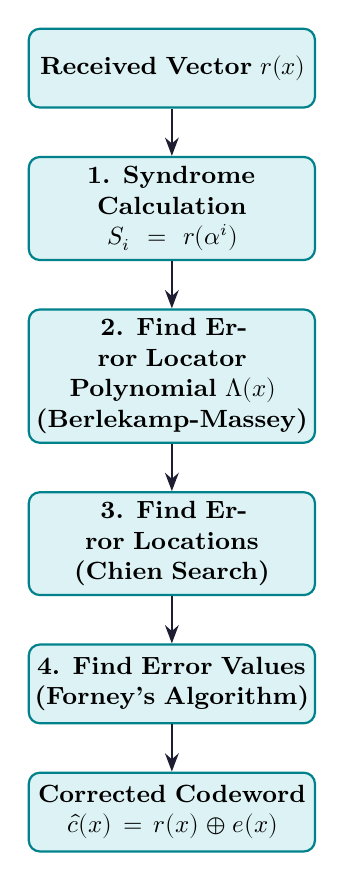
\begin{tikzpicture}[node distance=1.6cm]
  \node[stepnode] (n0) {Received Vector $r(x)$};
  \node[stepnode, below=0.6cm of n0] (n1) {1. Syndrome Calculation \\ $S_i = r(\alpha^i)$};
  \node[stepnode, below=0.6cm of n1] (n2) {2. Find Error Locator \\ Polynomial $\Lambda(x)$ \\ (Berlekamp-Massey)};
  \node[stepnode, below=0.6cm of n2] (n3) {3. Find Error Locations \\ (Chien Search)};
  \node[stepnode, below=0.6cm of n3] (n4) {4. Find Error Values \\ (Forney's Algorithm)};
  \node[stepnode, below=0.6cm of n4] (n5) {Corrected Codeword \\ $\hat{c}(x) = r(x) \oplus e(x)$};

  \draw[flowarrow] (n0) -- (n1);
  \draw[flowarrow] (n1) -- (n2);
  \draw[flowarrow] (n2) -- (n3);
  \draw[flowarrow] (n3) -- (n4);
  \draw[flowarrow] (n4) -- (n5);
\end{tikzpicture}
\end{tcolorbox}

% ===============================================================================
\section{Syndrome Polynomial and the Key Equation}
% ===============================================================================

Let $c(x)$ be the transmitted codeword polynomial, $r(x)$ be the received polynomial, and $e(x) = \sum_{j \in \mathcal{E}} Y_j x^j$ be the error polynomial, where $\mathcal{E}$ is the set of error positions and $Y_j$ are the error values ($Y_j \in \text{GF}(2)$ for binary BCH, and $Y_j \in \text{GF}(2^m)$ for RS codes).

\subsection{Syndrome Calculations}
The decoder calculates $2t$ syndromes:
\[ S_i = r(\alpha^i) = c(\alpha^i) \oplus e(\alpha^i) = 0 \oplus e(\alpha^i) = \sum_{l=1}^\nu Y_l X_l^i, \quad i = 1, 2, \dots, 2t \]
where $\nu$ is the actual number of errors, $X_l = \alpha^{i_l}$ is the \textbf{error locator} indicating the position of the $l$-th error, and $Y_l$ is the error value.
We define the \textbf{Syndrome Polynomial}:
\[ S(x) = \sum_{i=1}^{2t} S_i x^{i-1} = S_1 \oplus S_2 x \oplus S_3 x^2 \oplus \dots \oplus S_{2t} x^{2t-1} \]

\subsection{The Error Locator Polynomial}
The \textbf{Error Locator Polynomial} $\Lambda(x)$ has roots that are the reciprocals of the error locators $X_l$:
\begin{tcolorbox}[defbox, title={\textbf{Error Locator Polynomial}}]
\[ \Lambda(x) = \prod_{l=1}^\nu (1 - X_l x) = 1 + \Lambda_1 x + \Lambda_2 x^2 + \dots + \Lambda_\nu x^\nu \]
The roots of $\Lambda(x)$ are $x_l = X_l^{-1}$. Finding these roots reveals the error positions.
\end{tcolorbox}

\subsection{The Key Equation}
By defining the \textbf{Error Evaluator Polynomial} $\Omega(x)$ of degree less than $\nu$, we establish the fundamental relationship of algebraic decoding:
\begin{tcolorbox}[formulabox, title={\textbf{The Key Equation of Decoding}}]
\[ \Lambda(x) \cdot S(x) \equiv \Omega(x) \pmod{x^{2t}} \]
\end{tcolorbox}
The task of the decoder is to solve this equation for $\Lambda(x)$ and $\Omega(x)$, given the known syndrome polynomial $S(x)$.

% ===============================================================================
\section{The Berlekamp-Massey Algorithm}
% ===============================================================================

The \textbf{Berlekamp-Massey (BM)} algorithm is an iterative design procedure that solves the key equation. It views the syndrome values as outputs of a Linear Feedback Shift Register (LFSR) and finds the minimum register length $L$ and feedback connection polynomial $\Lambda^{(r)}(x)$ that can synthesize the sequence $S_1, S_2, \dots, S_{2t}$.

\subsection{Iterative Steps of the BM Algorithm}
We compute polynomials $\Lambda^{(r)}(x)$ for $r = 1, 2, \dots, 2t$:
\begin{tcolorbox}[formulabox, title={\textbf{Berlekamp-Massey Iteration}}]
At step $r$, we compute the \textbf{discrepancy} $d_r$:
\[ d_r = S_{r+1} \oplus \sum_{i=1}^L \Lambda_i^{(r)} S_{r+1-i} \]
\begin{enumerate}[leftmargin=*, itemsep=3pt, topsep=0pt]
  \item If $d_r = 0$, the current LFSR synthesizes the next syndrome:
    \[ \Lambda^{(r+1)}(x) = \Lambda^{(r)}(x), \quad L^{(r+1)} = L^{(r)} \]
  \item If $d_r \neq 0$, the loop coefficients must be adjusted:
    \[ \Lambda^{(r+1)}(x) = \Lambda^{(r)}(x) - d_r d_p^{-1} x^{r-p} \Lambda^{(p)}(x) \]
    where $p$ is a previous step that had a non-zero discrepancy $d_p$, chosen to minimize the new register length:
    \[ L^{(r+1)} = \max \left( L^{(r)}, \, r + 1 - L^{(r)} \right) \]
\end{enumerate}
\end{tcolorbox}
After $2t$ iterations, the resulting polynomial $\Lambda^{(2t)}(x)$ is the desired error locator polynomial $\Lambda(x)$.

% ===============================================================================
\section{Massey's Shift Register Synthesis}
% ===============================================================================

James Massey showed that the algebraic problem of decoding BCH codes is equivalent to the system-theoretic problem of synthesizing a minimum-length linear feedback shift register that generates a given sequence.

\begin{tcolorbox}[tikzbox, title={Massey's LFSR Synthesis Model}]
\centering
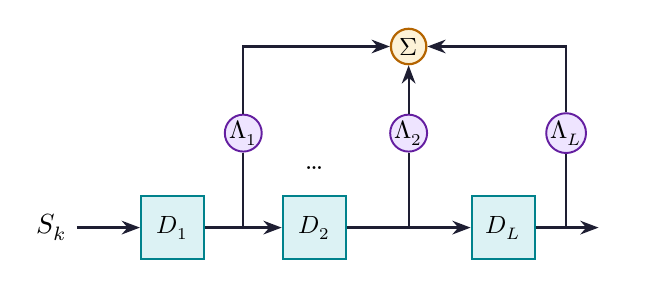
\begin{tikzpicture}[node distance=1.2cm]
  \node[reg] (s0) at (0,0) {$D_1$};
  \node[reg] (s1) at (1.8,0) {$D_2$};
  \node[reg] (s2) at (4.2,0) {$D_L$};

  \draw[arrow] (s0) -- (s1);
  \draw[arrow] (s1) -- (s2);

  \node[mult] (c1) at (0.9, 1.2) {$\Lambda_1$};
  \node[mult] (c2) at (3.0, 1.2) {$\Lambda_2$};
  \node[mult] (cL) at (5.0, 1.2) {$\Lambda_L$};

  \draw[line] (0.9, 0) -- (c1);
  \draw[line] (3.0, 0) -- (c2);
  \draw[line] (5.0, 0) -- (cL);

  \node[adder] (sum) at (3.0, 2.3) {$\Sigma$};
  \draw[arrow] (c1) |- (sum);
  \draw[arrow] (c2) -- (sum);
  \draw[arrow] (cL) |- (sum);

  \node[right=0.8cm of s2] (out) {};
  \draw[arrow] (s2) -- (out);

  \node[left=0.8cm of s0] (in) {$S_k$};
  \draw[arrow] (in) -- (s0);
  
  \node[above=0.2cm of s1] {\dots};
\end{tikzpicture}
\end{tcolorbox}

The feedback connections $\Lambda_1, \dots, \Lambda_L$ represent the coefficients of the error locator polynomial $\Lambda(x) = 1 + \Lambda_1 x + \dots + \Lambda_L x^L$. The discrepancy $d_r$ represents the difference between the actual syndrome $S_{r+1}$ and the output predicted by the shift register.

% ===============================================================================
\section{A Fast Berlekamp-Massey Algorithm}
% ===============================================================================

To handle high-speed data transmission (e.g., optical networks and solid-state storage), the iterative Berlekamp-Massey algorithm can be reorganized into a parallel, systolic architecture.
By utilizing division-free updates and maintaining auxiliary polynomials in parallel, modern decoders compute $\Lambda(x)$ in exactly $2t$ clock cycles without needing finite-field inversions ($d_p^{-1}$).

% ===============================================================================
\section{Chien Search and Forney's Algorithm}
% ===============================================================================

Once $\Lambda(x)$ and $\Omega(x)$ are computed, we must identify the error locations and calculate their values.

\subsection{Chien Search}
Chien search is a hardware-efficient method to find the roots of $\Lambda(x)$. Since the roots must lie in the finite field $\text{GF}(2^m)$, we test all possible elements $\alpha^{-i}$ ($i = 0, \dots, n-1$):
\[ \Lambda(\alpha^{-i}) = 1 + \Lambda_1 \alpha^{-i} + \Lambda_2 \alpha^{-2i} + \dots + \Lambda_\nu \alpha^{-\nu i} \]
If $\Lambda(\alpha^{-i}) = 0$, then position $i$ is identified as an error location.
In hardware, the terms $\Lambda_j \alpha^{-ji}$ are updated each clock cycle using simple scaling registers, avoiding expensive exponentiations.

\subsection{Forney's Algorithm}
For non-binary codes (like Reed-Solomon), we must find the error values $Y_l$ to correct the corrupted symbols. Forney's algorithm computes these directly:
\begin{tcolorbox}[formulabox, title={\textbf{Forney's Error Value Formula}}]
The error value $Y_l$ at position $i_l$ (where $X_l = \alpha^{i_l}$) is:
\[ Y_l = - \frac{\Omega(X_l^{-1})}{\Lambda'(X_l^{-1})} \]
where $\Lambda'(x)$ is the formal derivative of the error locator polynomial:
\[ \Lambda'(x) = \sum_{j=1}^\nu j \cdot \Lambda_j x^{j-1} \]
\end{tcolorbox}
In binary fields, the addition is modulo-2, so the negative sign is ignored, and the derivative $\Lambda'(x)$ simplifies to the sum of its odd-indexed terms.

% ═══════════════════════════════════════════════════════════════════════════════
% QUICK REVISION PAGE
% ═══════════════════════════════════════════════════════════════════════════════
\newpage
\begin{center}
  {\large\bfseries\color{myred} Quick Revision --- Module 4}\\[3pt]
  {\small\color{mydark} Decoding of BCH and RS Codes $|$ PE-EC801C}
\end{center}
\noindent{\color{myred}\rule{\linewidth}{1.2pt}}
\vspace{4pt}

\begin{tcolorbox}[formulabox, title={\textbf{Key Formulas and Metrics at a Glance}}]
\renewcommand{\arraystretch}{1.35}
\begin{tabularx}{\linewidth}{B{5.0cm} X}
Syndrome elements & $S_i = \sum_{l=1}^\nu Y_l X_l^i$ \\[4pt]
Syndrome Polynomial & $S(x) = \sum_{i=1}^{2t} S_i x^{i-1}$ \\[4pt]
Error Locator Polynomial & $\Lambda(x) = \prod_{l=1}^\nu (1 - X_l x)$ \\[4pt]
Key Equation of Decoding & $\Lambda(x) \cdot S(x) \equiv \Omega(x) \pmod{x^{2t}}$ \\[4pt]
Discrepancy equation & $d_r = S_{r+1} \oplus \sum_{i=1}^L \Lambda_i^{(r)} S_{r+1-i}$ \\[4pt]
Register length update & $L^{(r+1)} = \max \left( L^{(r)}, \, r + 1 - L^{(r)} \right)$ \\[4pt]
Chien search check & $\Lambda(\alpha^{-i}) = 0 \implies$ error at index $i$ \\[4pt]
Forney's error value & $Y_l = - \frac{\Omega(X_l^{-1})}{\Lambda'(X_l^{-1})}$ \\[4pt]
Formal derivative (binary) & $\Lambda'(x) = \Lambda_1 \oplus \Lambda_3 x^2 \oplus \Lambda_5 x^4 \oplus \dots$
\end{tabularx}
\end{tcolorbox}

\vspace{6pt}

\begin{tcolorbox}[defbox, title={\textbf{One-Line Definitions}}]
\begin{itemize}[leftmargin=*, itemsep=3pt, topsep=0pt]
  \item \textbf{Syndrome Polynomial ($S(x)$):} A polynomial constructed from received syndromes representing the error pattern.
  \item \textbf{Error Locator ($\Lambda(x)$):} A polynomial whose roots indicate the positions where transmission errors occurred.
  \item \textbf{Error Evaluator ($\Omega(x)$):} A polynomial containing spectral details used to calculate error magnitudes.
  \item \textbf{Discrepancy ($d_r$):} The difference between the observed syndrome and the LFSR prediction in BM.
  \item \textbf{Berlekamp-Massey Algorithm:} An iterative, FSR-based procedure used to solve the key equation.
  \item \textbf{Chien Search:} A systematic search method evaluating $\Lambda(x)$ at all field elements to find roots.
  \item \textbf{Forney's Algorithm:} A low-complexity algebraic method used to calculate error values for non-binary codes.
  \item \textbf{Key Equation:} The core modular relationship linking $\Lambda(x)$, $S(x)$, and $\Omega(x)$ in algebraic decoding.
\end{itemize}
\end{tcolorbox}

\newpage

\begin{tcolorbox}[exambox, title={\textbf{Frequently Asked / Viva Questions}}]
\begin{enumerate}[topsep=0pt, label=\textbf{Q\arabic*.}, itemsep=5pt]
  \item \Q{What are the four main steps of the BCH/RS decoding pipeline?}
    First, compute the syndrome values from the received vector. Second, apply the Berlekamp-Massey algorithm to compute the error locator polynomial $\Lambda(x)$. Third, perform Chien search to find the roots of $\Lambda(x)$, locating the errors. Fourth, use Forney's algorithm to compute error values.
  \item \Q{State the Key Equation of decoding and define its terms.}
    The Key Equation is $\Lambda(x) \cdot S(x) \equiv \Omega(x) \pmod{x^{2t}}$, where $\Lambda(x)$ is the error locator polynomial, $S(x)$ is the syndrome polynomial, and $\Omega(x)$ is the error evaluator polynomial. It links the time and spectral representations of errors.
  \item \Q{How does the Berlekamp-Massey algorithm model the decoding problem?}
    The BM algorithm models the syndrome sequence as outputs of a Linear Feedback Shift Register (LFSR). It iteratively constructs the shortest LFSR that generates the syndromes, which represents the minimum-degree error locator.
  \item \Q{Explain the concept of 'discrepancy' in the BM algorithm.}
    Discrepancy ($d_r$) is the difference between the actual syndrome $S_{r+1}$ and the value predicted by the feedback connections of the current iteration. If $d_r = 0$, the connections are correct; if $d_r \neq 0$, the connection polynomial must be adjusted.
  \item \Q{What is Chien search, and how does it optimize hardware implementation?}
    Chien search finds the roots of $\Lambda(x)$ by evaluating it at all field elements $\alpha^{-i}$. In hardware, terms are updated using multipliers that scale by constant values (powers of $\alpha$), replacing complex exponentiations with simple shifts.
  \item \Q{Explain Forney's algorithm and why it is useful.}
    Forney's algorithm calculates error values using $Y_l = -\Omega(X_l^{-1})/\Lambda'(X_l^{-1})$. It is highly useful because it allows direct computation of error values at known error locations without solving a large system of simultaneous equations.
  \item \Q{Why does the formal derivative of a polynomial simplify in binary fields?}
    In binary fields, addition is modulo-2. Since $2 \equiv 0 \pmod 2$, all terms with even powers in the derivative disappear (since their derivatives contain an even multiplier: $2 \cdot c \cdot x = 0$). Thus, only the odd-indexed terms remain.
  \item \Q{Can the BM algorithm handle erasure decoding?}
    Yes. Erasures are errors with known locations but unknown values. The BM algorithm can be initialized with an erasure locator polynomial, reducing the number of syndrome iterations needed to solve for the remaining unknown errors.
  \item \Q{What is the difference between Berlekamp-Massey and the Euclidean decoding algorithm?}
    BM is an iterative LFSR design process that runs in $2t$ steps. The Euclidean algorithm solves the key equation by finding the greatest common divisor of $x^{2t}$ and $S(x)$ using polynomial division. Both produce identical results.
  \item \Q{What happens during decoding if the number of channel errors exceeds $t$?}
    If the number of errors exceeds $t$, the Berlekamp-Massey algorithm will still compute a polynomial, but it will have invalid roots, or the roots won't correspond to correct locations, resulting in a decoding failure or undetected error.
\end{enumerate}
\tcbset{after={\color{black}}}
\end{tcolorbox}

\vspace{6pt}

\begin{tcolorbox}[tikzbox, title={\textbf{Comparison of Decoding Algorithms}}]
\renewcommand{\arraystretch}{1.45}
\begin{tabularx}{\linewidth}{|B{3.2cm}|Y|Y|}
\hline
\textbf{Property} & \textbf{Berlekamp-Massey Algorithm} & \textbf{Euclidean Algorithm} \\
\hline
Mathematical Basis & Linear feedback shift register synthesis & Polynomial GCD division \\
\hline
Execution Flow & Iterative (updates loop coefficients) & Recursive division steps \\
\hline
Hardware Suitability & Excellent (systolic array architectures) & Challenging (requires polynomial dividers) \\
\hline
Design Focus & Solving the LFSR feedback connections & Direct fraction reduction of $S(x)/x^{2t}$ \\
\hline
\end{tabularx}
\end{tcolorbox}

\end{document}
